% ============================================================================
% CHAPTER 3: PROPOSED ALGORITHM INTRODUCTION
% ============================================================================

\chapter{معرفی الگوریتم پیشنهادی}

\section{مقدمه}
در این فصل، ساختار دقیق الگوریتم پیشنهادی مبتنی بر ۹ سیستم آشوبی نمایی و سیستم \lr{Chen} تشریح می‌شود. الگوریتم پیشنهادی در شکل نهایی خود به‌گونه‌ای تدوین شده که تمامی مؤلفه‌های نظری در آن نهادینه شده‌اند.

\section{الگوریتم پیشنهادی}
الگوریتم پیشنهادی از یک فرآیند دو مرحله‌ای شامل جایگشت (\lr{Permutation}) و انتشار (\lr{Diffusion}) تشکیل شده است. نوآوری اصلی این روش در استفاده از انتخاب‌گر دینامیک برای ۹ نگاشت آشوبی نمایی است.

\section{مدل آشوبی نمایی (\lr{ECM})}
مدل آشوبی نمایی با ترکیب نگاشت‌های پایه و اعمال توان نمایی ایجاد می‌شود. در این پژوهش ۹ ترکیب مختلف (\lr{LEL}, \lr{LES}, \lr{LET}, \dots) استفاده شده است.

\begin{figure}[h]
    \centering
    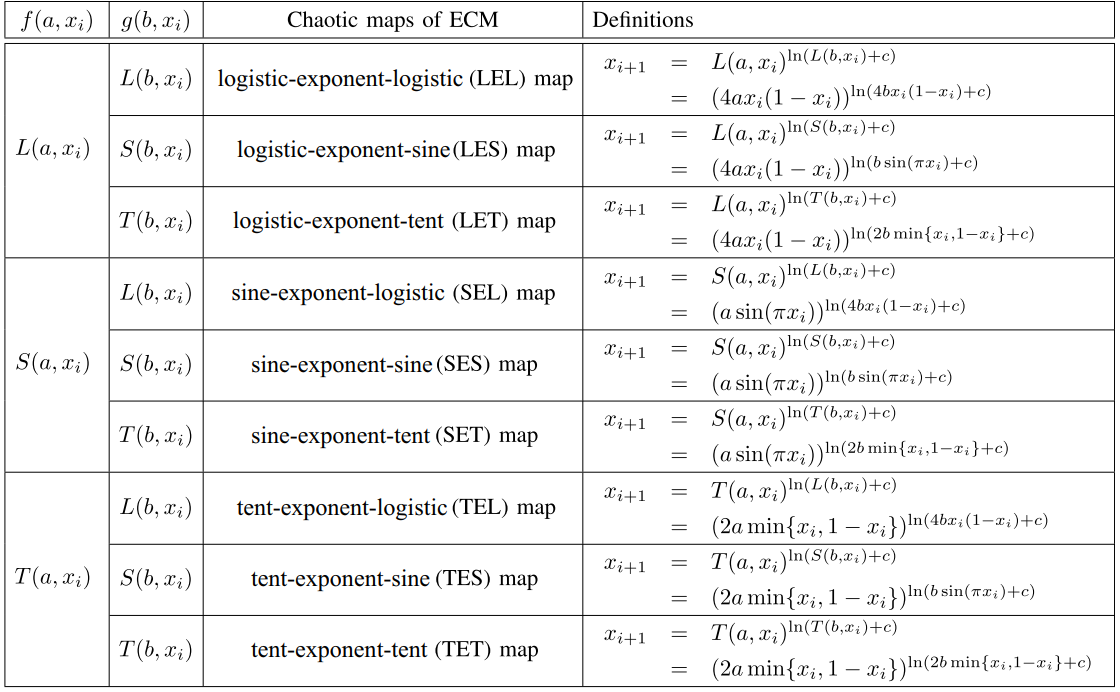
\includegraphics[width=0.8\textwidth]{vertopal_6a6e478acc1947c1bfecfac3523ed62b/media/image10}
    \caption{ساختار ۹ سیستم آشوبی نمایی ترکیبی}
\end{figure}

\section{فرآیند رمزنگاری}
فرآیند رمزنگاری در پنج مرحله اصلی انجام می‌شود: تولید کلیدهای اولیه، جایگشت پیکسل‌ها با سیستم \lr{Chen}، رمزنگاری با انتخاب‌گر دینامیک، انتشار مقادیر رنگی و ترکیب نهایی.

\section{تحلیل ساختاری مراحل پیاده‌سازی}

\subsection{تولید مسیرهای آشوبی مبتنی بر سیستم \lr{Chen}}
سیستم \lr{Chen} از جمله سیستم‌های سه‌بعدی ابرجاذبی است که حساسیت بسیار بالایی به شرایط اولیه دارد. معادلات حاکم بر این سیستم عبارتند از:
\begin{equation}
\begin{cases}
    \dot{x} = a(y-x) \\
    \dot{y} = (c-a)x - xz + cy \\
    \dot{z} = xy - bz
\end{cases}
\end{equation}

\subsection{تولید بردار جایگشت}
پس از نرمال‌سازی خروجی‌ها، بردارهای جایگشت یک‌به‌یک تولید می‌شود که موجب تخریب کامل ساختار هندسی تصویر می‌گردد.

\subsection{انتشار مبتنی بر \lr{XOR}}
دنباله‌های بایت‌های تولیدشده به‌صورت مستقیم در عملیات \lr{XOR} با پیکسل‌های جایگشت‌شده به‌کار گرفته می‌شوند. این مرحله عامل اصلی مقاومت در برابر حملات تفاضلی است.

\subsection{رمزگشایی معکوس}
از آنجا که عملیات \lr{XOR} و جایگشت برگشت‌پذیر هستند، تصویر اصلی بدون هیچ‌گونه خطا بازیابی می‌شود (\lr{Lossless recovery}). معکوس‌پذیری کامل الگوریتم تضمین شده است.
\
